\documentclass[main]{subfiles}
\begin{document}

%@@@@@@@@@@@@@@@@@@@@@@@@@@@@@@
%\noindent
%\textbf{Topic: Hopfield Networks - 26.11.2020} \\
%Lecturer: Dr. Matthew Cook \\
%Author: Vanessa Leite \{vanessa at ini.uzh.ch\}

\section{Hopfield Networks}

The Hopfield Network, or Hopfield Model, was proposed by John Hopfield in the early 80s.
He was trying to understand what neural networks do.
When we look into the brain and how neurons are connected to each other, we do not see always a clear pathway, i.e., it is hard to think about the connections in the brain in terms of input-output.
He thought about connecting units to each other in an all-to-all pattern and see what would happen.

\paragraph{Characteristics of Hopfield Networks}
\begin{itemize}[noitemsep,nolistsep]
	\item Every node is connected to every other node but not to itself.
	\item Connection weights are symmetric (bidirectional).
	\item $\sum x_i w_i < 0$ represents an inactive unit, $\sum x_i w_i \geq 0$ is active, when using a zero threshold.
	\item The entire network is in some state at any time. Set of active units of the entire network is important.
	\item Some states are stable and some are not. While in an unstable state, updating the network leads to a state change.
	\item Stable state is a local minimum.
	\item Bias is an unit that is always on.
	\item Weight symmetry of a connection is correlated to the frequency of neurons firing together (following Hebbian learning).
\end{itemize}

\subsection{Hopfield and Memory}

We are used to think about computation as a process that receives an input, does something and generates an output.
However, this is not what we ``see" in the memory process, for instance.
It seems our memory works with Pattern Completion, also known as Content Addressable Memory or Associative Memory.
This memory has no input-output relation: given any piece of it, we can recover the rest.
An example is when certain smell can bring us a memory, even though the smell is only part of the memory.
Hopfield Networks can be used to give us insights about how the memory works by having a highly connected network that computes with no input-output, but with states.
The network has some dynamics that \"walk" through a state space, i.e., the space of all the possible states. The Hopfield Network is dynamic and moves from one state to another until it arrives to a stable state (also known as an attractor). Having stable states help the network to recover information giving partial inputs.


\begin{itemize}[noitemsep,nolistsep]
	\item A Hopfield Network is an associative type of memory. Information is stored in the stable states as local minima.
	\item It is important that information is distinct.
	\item Associative memory has room for error but is still recognizable. Convergence to nearby stable states.
	\item If some units are retrievable and all others are set randomly, the correct units will eventually set the wrong units right.
\end{itemize}

\begin{figure}[H]
	\centering
	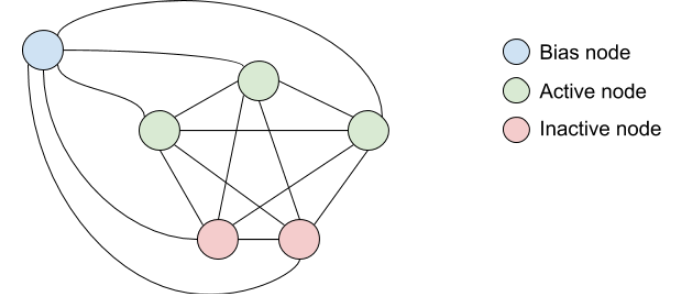
\includegraphics[width=0.5\textwidth]{hopfield-network-basic.png}
	\caption{Model of a Hopfield Network. Red units are inactive, green units are active, blue unit is the bias node that is always active.}
\end{figure}

\subsection{Updates and State Dynamics}

Hopfield found that these networks always converge to a stable state.
Idea: Consider the sum of weights between active units ($Q$).
The update rule is equivalent to always increase $Q$, i.e., we turn an unit active if $\sum x_i w_i >= \theta$, where $x_i$ is the value of the state of each unit, $w_i$ is the weight between the units and $\theta$ is the threshold, thus maximizing $Q$ (weights between active units) by updating the output of one unit at time (see Figure~\ref{fig:asynchronous-update}).
In this setup, the update algorithm of Hopfield Networks can be seen as a greedy algorith to find the MAX-CLIQUE.
We update all the units but the bias node (bias node are always active and do not change their state).
Remember, inactive neurons with zero threshold don't send inhibitory signal, instead they do not take part in the activation of other neurons.

\begin{figure}[H]
	\centering
	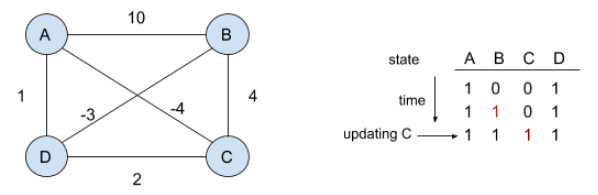
\includegraphics[width=0.8\textwidth]{asynchronous-update-hopfield.png}
	\caption{Hopfield network model, asynchronous updates and greedy algorith to find MAX-CLIQUE}
	\label{fig:asynchronous-update}
\end{figure}

Consider the network presented in Figure~\ref{fig:asynchronous-update}: states are in the table on the right.
In the beggining A and D are active, the sum of the active weights ($Q$) is 1.
Now, we look at B and we sum the weights of the active units linked to B (D and A).
$Q$ is ($10 - 3 = 7 >= 0$).
If $Q \geq 0$ we put the unit on the top part (unit active), otherwise we put the unit on the bottom (unit inactive), see Figure~\ref{fig:sum-weights}.
If B becomes active, $Q$ increases (sum = 1 + 7).
If B becomes inactive, $Q$ does not change (sum = 1).
After updating C, the network achieves a stable state, i.e., updating any unit does not change its output.

\begin{figure}[H]
	\centering
	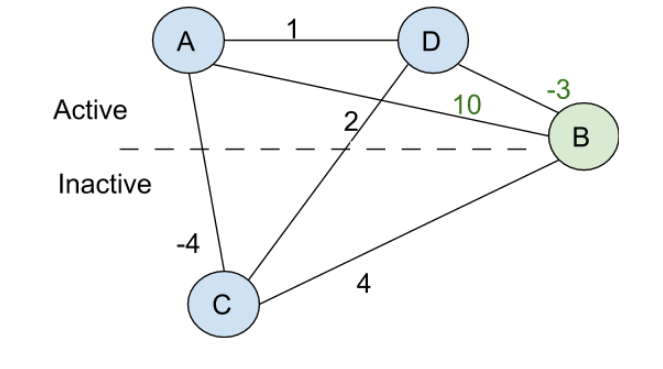
\includegraphics[width=0.5\textwidth]{sum-weights-active-units.png}
	\caption{Evaluation of node B}
	\label{fig:sum-weights}
\end{figure}

When we update a unit and change its value (active or inactive), then $Q$ increases or stays the same (if we are making units active). When we make units inactive, $Q$ doesnt change.
We can also consider active units as having a value of ``$+1$'' and inactive units as a ``$-1$''.
In this new representation, the Hopfield Network dynamic is equivalent to a graph min-cut, i.e., we want to minimize the sum of weights that link active and inactive units.

\paragraph{Asynchronous updates}
When we update one unit at time, we are using an asynchronous method.
Asynchronous Hopfield Networks always converge to a stable state, regardless of the update order, however, to which stable state is dependent on the update order, see Figure~\ref{fig:hopfield-order-update}.

\begin{figure}[H]
	\centering
	\includegraphics[width=0.7\textwidth]{hopfield-order-update.png}
	\caption{Considering a Hopfield network with two units connected with weight $= 2$, threshold zero, and a bias unit of $-1$. Starting in a state with 1 active and 2 inactive, we can see how the order of update can lead to different stable states.
	By updating first unit $1$ then unit $2$, the stable state is with both units inactive. However, updating unit $2$ then unit $1$, we arrive to a stable state where both units are active.}
	\label{fig:hopfield-order-update}
\end{figure}

\paragraph{Synchronous updates}
Let's now consider a synchronous case, i.e., when we update all units at the same time: for this, active units for time $t+1$ are computed based on active units at time $t$.
In this case, the system becomes a deterministic system because it doesn't depend on the order of updates anymore.
Consider the network on Figure~\ref{fig:synchronous-hopfield}, starting with units $1$ and $2$ active, in the next step of update (after all units), unit $3$ and $4$ should be active. It may be confusing to see this by updating one unit per time, let's say we update units in the order${1, 2, 3, 4}$: after updating unit $3$ it will become active but, when updating unit $4$, we shouldn't consider unit $3$, yet.

\begin{figure}[H]
	\centering
	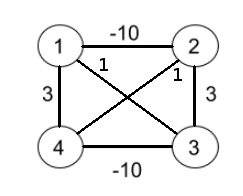
\includegraphics[width=0.3\textwidth]{synchronous-hopfield.png}
	\caption{Starting with 1 and 2 actives, in the next step 3 and 4 will be active. This network doesn't have a unique stable state but converges to a cycle between two states.}
	\label{fig:synchronous-hopfield}
\end{figure}

Trick for analysis: make a larger asynchronous network based on the network we want to analyse. Duplicate the units in two columns and only use non-zero weights between them.

\begin{figure}[H]
	\centering
	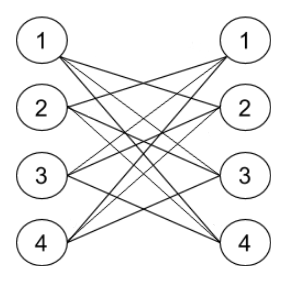
\includegraphics[width=0.3\textwidth]{hopfield-asynchronous-trick.png}
	\caption{Starting with 1 and 2 actives, we will end up with 3 and 4 active in the second column. First column represents $t=0$, second $t=1$. With synchronous updates, a Hopfield Network converges to a cycle of length 2 or to a stable state.}
\end{figure}

\paragraph{Summary}
\begin{itemize}[noitemsep,nolistsep]
	\item Nodes can be updated synchronously or asynchronously.
	\item State: Set of units that are active, it can be seen as the activity vector.
	\item Dynamics: Units update their activity level.
	\item When a node is updated, weights are considered from all other active nodes, like with a perceptron.
	\item Asynchronous updates (greedy algorithm) converge to a stable state (sequential), but the converged state can depend on update order.
	\item Asynchronous is either in max-clique state if activity is in $\{0,1\}$ or min-cut if activities are in $\{-1,1\}$.
	\item Synchronous, parallel updates either also go to a stable state, just like asynchronous, or can get stuck in a pair of patterns (flipping or cyclic).
\end{itemize}

%\subsection{Hebbian learning in Hopfield Networks}
%Learning the network weights that lead to a stable pattern can be implemented using Hebbian Learning.
%We update the network's weight (initially set to zero) in each iteraction according to the rule:
%$w_{ij} \leftarrow w_{ij} + x_i^k x_j^k$, $i\neq j$.\\
%Where $x_i^k$ and $x_j^k$ denote the $i-$th and $j-$th component respectively of each vector $x_k$, and $k$ is the number of patterns that we want to learn.
%
%Consider that we want to learn the patterns: $x_1 = [ -1, 1, 1, -1]$ and $x_2 = [-1, 1, -1, 1]$.
%The initial weight matrix of the network is:
%\[
%W = 
%\begin{pmatrix}
%0 & 0 & 0 & 0\\
%0 & 0 & 0 & 0\\
%0 & 0 & 0 & 0\\
%0 & 0 & 0 & 0
%\end{pmatrix}
%\]
%Then we present the first pattern to be learn, i.e., update all weights using the mentioned rule.
%This way, for instance, $w_{12} = \underbrace{0}_{\text{previous weight}} + \underbrace{(-1)}_{\text{first element in $x_1$}}\times \overbrace{(1)}^{\text{second element in $x_1$}}$.
%
%After the presentation of all the components of the first pattern, we will have: $W_1 = x_1^T x_1 - I$. We subtract the identity matrix to impose that the diagonal of $W$ has zero entries.
%\[
%W_1 = 
%\begin{pmatrix}
%0 & -1 & -1 & 1\\
%-1 & 0 & 1 & -1\\
%-1 & 1 & 0 & -1\\
%1 & -1 & -1 & 0
%\end{pmatrix}
%\]
%
%After the presentation of the second pattern: $W_2 = W_1 + x_2^T x_2 - I$.
%
%\[
%W_2 = 
%\begin{pmatrix}
%0 & -2 & 0 & 0\\
%-2 & 0 & 0 & 0\\
%0 & 0 & 0 & -2\\
%0 & 0 & -2 & 0
%\end{pmatrix}
%\]
%
%Because $w_{ij} \neq 0$ in Hopfield networks, we cannot use this solution. We would find a solution only by applying the perceptron learning algorithm.

\end{document}
